\documentclass[aspectratio=169]{beamer}

\definecolor{red}{RGB}{220, 50, 47}
\definecolor{green}{RGB}{133, 153, 0}
\definecolor{cyan}{RGB}{42, 161, 152}
\definecolor{blue}{RGB}{38, 139, 210}
\definecolor{yellow}{RGB}{181, 137, 0}

% Suppress all navigation symbols
\setbeamertemplate{navigation symbols}{}
\setbeamertemplate{headline}{}
\setbeamertemplate{footline}{}
\setbeamertemplate{itemize items}[circle]
\setbeamertemplate{footline}[frame number]

\setbeamercolor{structure}{fg=blue}
\setbeamercolor{normal text}{fg=black, bg=white}
\setbeamerfont{title}{series=\bfseries}
\setbeamerfont{frametitle}{series=\bfseries}

\usepackage{fontspec}
\setmainfont[Ligatures=TeX]{Tinos}
\setsansfont{Arimo}[Scale=MatchLowercase]
\setmonofont{Cousine}[Scale=MatchLowercase]

\usepackage{tikz}
\usetikzlibrary{arrows}
\usetikzlibrary{calc}
\usetikzlibrary{positioning}
\usetikzlibrary{matrix}
\usetikzlibrary{shapes}

\title{C++ const and Immutability: An Empirical Study of
       Writes-Through-const}
\author{Jon Eyolfson}
\date{2016-07-20}

\newcommand{\const}{{\color{blue} \bfseries \ttfamily const}}

\setbeamertemplate{title page}
{
  \begin{tikzpicture}[remember picture,
                      overlay,
                      shift={(current page.south west)}]
    \node (title) [inner sep=0, scale=1.5, align=left]
          at (\paperwidth / 3, \paperheight / 2)
          {\usebeamerfont{title}\usebeamercolor[fg]{title}C++ \const{} and\\
           \usebeamerfont{title}\usebeamercolor[fg]{title}Immutability:\\
           \usebeamerfont{title}\usebeamercolor[fg]{title}An Empirical\\
           \usebeamerfont{title}\usebeamercolor[fg]{title}Study of Writes-\\
           \usebeamerfont{title}\usebeamercolor[fg]{title}Through-\const{}};
    \node at (\paperwidth * 2 / 3, \paperheight * 2 / 3) {\insertauthor};
    \node at (\paperwidth * 2 / 3, \paperheight / 3) {\insertdate};
  \end{tikzpicture}
}

\newlength{\barlength}
\setlength{\barlength}{10cm}

\newcommand{\transition}[1]{
  \begin{frame}
    \begin{center}
      \usebeamerfont{title}\usebeamercolor[fg]{title}#1
    \end{center}
  \end{frame}
}

\tikzset{
  every matrix/.style={
    fill=black!20,
    inner sep=2mm, row sep=0.5mm,
    matrix of nodes, nodes in empty cells,
    minimum height=0.5em, minimum width=.75em,
    nodes={anchor=base, inner sep=0, font=\ttfamily},
    ampersand replacement=\&
  },
  arrow/.style={->,>=stealth',shorten >=1mm, shorten <=1mm, thick}
}

\begin{document}

  \begin{frame}[plain]
    \titlepage
  \end{frame}

  \begin{frame}
    \frametitle{Immutability}
    \centering
    
\begin{tikzpicture}
      \node [draw=red, line width=3mm, forbidden sign, font=\Huge,
             minimum size=25mm, scale=2]
        {Writes};
    \end{tikzpicture}
  \end{frame}

  \begin{frame}
    \frametitle{The Caller Expects \texttt{C} to not Change}
    \centering
    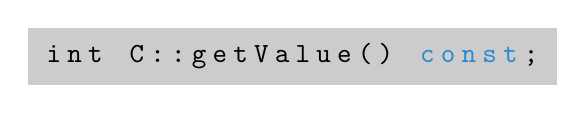
\begin{tikzpicture}
      \matrix (decl) {
        i \& n \& t \&   \& C \& : \& : \& g \& e \& t \& V \& a \& l \& u \&
        e \& ( \& ) \&   \& |[blue]|c \& |[blue]|o \& |[blue]|n \& |[blue]|s \&
        |[blue]|t \& ; \\
      };
    \end{tikzpicture}
  \end{frame}

  \begin{frame}
    \frametitle{C++ \const{} and Immutability}
    \Large
    C++ has some notion of immutability in the language

    \vspace{1em}
    \const{} represents \structure{shallow} physical immutability

    \vspace{1em}
    Shallow immutability does not allow fields to change
  \end{frame}

  \begin{frame}
    \frametitle{We Assume \const{} Means Deep Physical Immutability}
    \Large

    \structure{Deep} immutability does not allow changes through fields

    \vspace{1em}
    This is the most restrictive form of immutability

    \vspace{1em}
    A write-through-\const{} is a violation of deep immutability
  \end{frame}

  \begin{frame}
    \frametitle{Research Question 1: Do developers write-though-\const{}?}
    \Large

    Yes, they violate shallow and \structure{deep} immutability
  \end{frame}

  \begin{frame}
    \frametitle{Research Question 2: How developers write-though-\const{}?}
    \Large

    Either by using \texttt{mutable} or transitively through fields
  \end{frame}

  \begin{frame}
    \frametitle{Research Question 3: Why do developers write-though-\const{}?}
    \Large
    Conventional wisdom is for buffering / caching

    \vspace{1em}
    We found \structure{around half} are for invalid reasons
  \end{frame}

  \begin{frame}
    \frametitle{Physical Immutability}
    \centering
    \large
    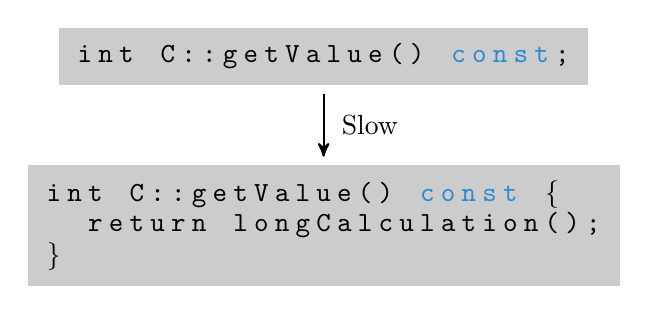
\begin{tikzpicture}
      \matrix (decl) {
        i \& n \& t \&   \& C \& : \& : \& g \& e \& t \& V \& a \& l \& u \&
        e \& ( \& ) \&   \& |[blue]|c \& |[blue]|o \& |[blue]|n \& |[blue]|s \&
        |[blue]|t \& ; \\
      };


      \matrix (defn) [below=of decl] {
        i \& n \& t \&   \& C \& : \& : \& g \& e \& t \& V \& a \& l \& u \&
        e \& ( \& ) \&   \& |[blue]|c \& |[blue]|o \& |[blue]|n \& |[blue]|s
        \& |[blue]|t \&   \& \{ \& \& \\

  \&   \& r \& e \& t \& u \& r \& n \&   \& l \& o \& n \& g \& C \& a \& l \& c \& u \& l \& a \& t \& i \& o \& n \& ( \& ) \& ; \\
\} \&   \&   \&   \&   \&   \&   \&   \&   \&   \&   \&   \&   \&   \&   \&   \&   \&   \&   \&   \&   \&   \&   \&   \&   \&   \&   \\
  };

      \draw [arrow] (decl) -- node [right, xshift=1mm] {Slow} (defn);
    \end{tikzpicture}
  \end{frame}

  \begin{frame}
    \frametitle{Abstract Immutability}
    \large
    \centering
    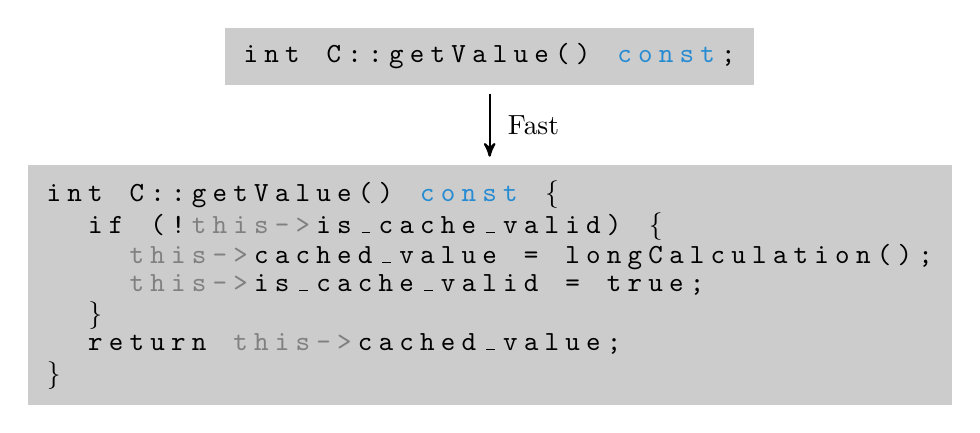
\begin{tikzpicture}
      \matrix (decl) {
        i \& n \& t \&   \& C \& : \& : \& g \& e \& t \& V \& a \& l \& u \&
        e \& ( \& ) \&   \& |[blue]|c \& |[blue]|o \& |[blue]|n \& |[blue]|s \&
        |[blue]|t \& ; \\
      };

      \matrix (defn) [below=of decl] {
i \& n \& t \&   \& C \& : \& : \& g \& e \& t \& V \& a \& l \& u \& e \& ( \& ) \&   \& |[blue]|c \& |[blue]|o \& |[blue]|n \& |[blue]|s \& |[blue]|t \&   \& \{ \&   \&   \&   \&   \&   \&   \&   \&   \&   \&   \&   \&   \&   \&   \&   \&   \&   \&   \\
  \&   \& i \& f \&   \& ( \& ! \& |[black!50]|t \& |[black!50]|h \& |[black!50]|i \& |[black!50]|s \& |[black!50]|- \& |[black!50]|> \& i \& s \& \_ \& c \& a \& c \& h \& e \& \_ \& v \& a \& l \& i \& d \& ) \&   \& \{ \&   \&   \&   \&   \&   \&   \&   \&   \&   \&   \&   \&   \&   \\
  \&   \&   \&   \& |[black!50]|t \& |[black!50]|h \& |[black!50]|i \& |[black!50]|s \& |[black!50]|- \& |[black!50]|> \& c \& a \& c \& h \& e \& d \& \_ \& v \& a \& l \& u \& e \&   \& = \&   \& l \& o \& n \& g \& C \& a \& l \& c \& u \& l \& a \& t \& i \& o \& n \& ( \& ) \& ; \\
  \&   \&   \&   \& |[black!50]|t \& |[black!50]|h \& |[black!50]|i \& |[black!50]|s \& |[black!50]|- \& |[black!50]|> \& i \& s \& \_ \& c \& a \& c \& h \& e \& \_ \& v \& a \& l \& i \& d \&   \& = \&   \& t \& r \& u \& e \& ; \&   \&   \&   \&   \&   \&   \&   \&   \&   \&   \&   \\
  \&   \& \} \&   \&   \&   \&   \&   \&   \&   \&   \&   \&   \&   \&   \&   \&   \&   \&   \&   \&   \&   \&   \&   \&   \&   \&   \&   \&   \&   \&   \&   \&   \&   \&   \&   \&   \&   \&   \&   \&   \&   \&   \\
  \&   \& r \& e \& t \& u \& r \& n \&   \& |[black!50]|t \& |[black!50]|h \& |[black!50]|i \& |[black!50]|s \& |[black!50]|- \& |[black!50]|> \& c \& a \& c \& h \& e \& d \& \_ \& v \& a \& l \& u \& e \& ; \&   \&   \&   \&   \&   \&   \&   \&   \&   \&   \&   \&   \&   \&   \&   \\
\} \&   \&   \&   \&   \&   \&   \&   \&   \&   \&   \&   \&   \&   \&   \&   \&   \&   \&   \&   \&   \&   \&   \&   \&   \&   \&   \&   \&   \&   \&   \&   \&   \&   \&   \&   \&   \&   \&   \&   \&   \&   \&   \\
      };
      \draw [arrow] (decl) -- node [right, xshift=1mm] {Fast} (defn);
    \end{tikzpicture}
  \end{frame}

  \begin{frame}
    \frametitle{Type System Only Approachs are Restrictive}
    \Large
    Abstract immutability is either:

    \begin{itemize}
      \item Unsupported
      \item Unchecked
    \end{itemize}
  \end{frame}

  \begin{frame}
    \frametitle{Incorrect \const{} Methods Lead to Errors}
    \Large
    Hashmap
  \end{frame}

  \begin{frame}
    \frametitle{Technique Overview}

    \begin{enumerate}
      \item C++ additional metadata
      \item LLVM instrumentation
      \item Runtime library
    \end{enumerate}
  \end{frame}

  \begin{frame}
    \frametitle{Technique}
    \Large
    Report writes through \const{} that are unchecked by compiler

    Also follow writes though \const{} cast (sledgehammer)
  \end{frame}

  \begin{frame}
    \frametitle{Technique}
    \Large
    Shadow values with example

    Arguments are passed through TLS
  \end{frame}

  \begin{frame}
    \frametitle{How?}
    \Large

    Transitive

    Mutable

    \const{} cast
  \end{frame}

  \begin{frame}
    \frametitle{Reasons for Writes Through Immutable Declarations}
    \Large
    \begin{itemize}
      \item Buffer / caching
      \item Delayed initialization
      \item Incorrect (around {\color{blue} half}!)
    \end{itemize}

    Additional:
    \begin{itemize}
      \item Not visible (not accessible through public API)
      \item Synchronization
    \end{itemize}
  \end{frame}

  \begin{frame}
    \frametitle{Results Overview}
    \Large
    Overview of projects
  \end{frame}

  \begin{frame}
    \frametitle{Not Visible Example}
    \centering
    \large
    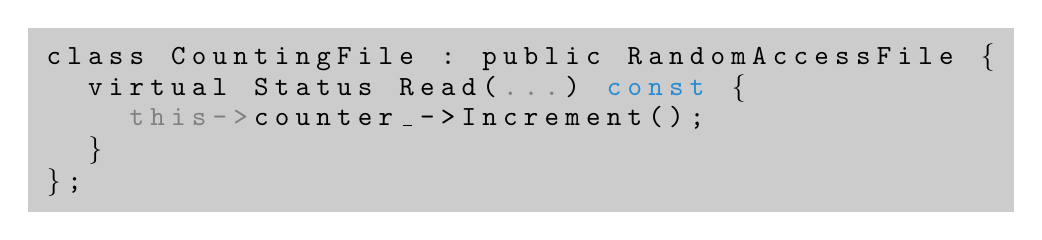
\begin{tikzpicture}
  \matrix  {
c \& l \& a \& s \& s \&   \& C \& o \& u \& n \& t \& i \& n \& g \& F \& i \& l \& e \&   \& : \&   \& p \& u \& b \& l \& i \& c \&   \& R \& a \& n \& d \& o \& m \& A \& c \& c \& e \& s \& s \& F \& i \& l \& e \&   \& \{ \\
  \&   \& v \& i \& r \& t \& u \& a \& l \&   \& S \& t \& a \& t \& u \& s \&   \& R \& e \& a \& d \& ( \& |[black!50]|. \& |[black!50]|. \& |[black!50]|. \& ) \&   \& |[blue]|c \& |[blue]|o \& |[blue]|n \& |[blue]|s \& |[blue]|t \&   \& \{ \&   \&   \&   \&   \&   \&   \&   \&   \&   \&   \&   \&   \\
  \&   \&   \&   \& |[black!50]|t \& |[black!50]|h \& |[black!50]|i \& |[black!50]|s \& |[black!50]|- \& |[black!50]|> \& c \& o \& u \& n \& t \& e \& r \& \_ \& - \& > \& I \& n \& c \& r \& e \& m \& e \& n \& t \& ( \& ) \& ; \&   \&   \&   \&   \&   \&   \&   \&   \&   \&   \&   \&   \&   \&   \\
  \&   \& \} \&   \&   \&   \&   \&   \&   \&   \&   \&   \&   \&   \&   \&   \&   \&   \&   \&   \&   \&   \&   \&   \&   \&   \&   \&   \&   \&   \&   \&   \&   \&   \&   \&   \&   \&   \&   \&   \&   \&   \&   \&   \&   \&   \\
\} \& ; \&   \&   \&   \&   \&   \&   \&   \&   \&   \&   \&   \&   \&   \&   \&   \&   \&   \&   \&   \&   \&   \&   \&   \&   \&   \&   \&   \&   \&   \&   \&   \&   \&   \&   \&   \&   \&   \&   \&   \&   \&   \&   \&   \&   \\
  };
    \end{tikzpicture}
  \end{frame}

  \begin{frame}
    \frametitle{Protobuf's Unique Archetypes}
    \Large
    \begin{tabular}{p{2.65cm} p{4cm} c c}
      \textbf{Root Cause} & \textbf{Main Attribute}
      & \textbf{Not visible?} & \textbf{Synchronized?} \\

      Transitive & Buffer/Cache & Yes & Yes \\
      \texttt{mutable} & Buffer/Cache &   & Yes \\
      Transitive & Incorrect &   &   \\
      \texttt{mutable} & Incorrect &   & Yes \\
      \texttt{mutable} & Delayed Initialization & Yes & Yes \\
      & & & \\
    \end{tabular}
  \end{frame}

  \begin{frame}
    \frametitle{LevelDB's Unique Archetypes}
    \Large
    \begin{tabular}{p{2.65cm} p{4cm} c c}
      \textbf{Root Cause} & \textbf{Main Attribute}
      & \textbf{Not visible?} & \textbf{Synchronized?} \\

      Transitive & Unit Testing & Yes & Yes \\
      Transitive & Buffer/Cache &   & Yes \\
      Transitive & Incorrect &   &   \\
      Transitive & Incorrect &   &   \\
      Transitive & Incorrect &   & Yes \\
      Transitive & Unit Testing & Yes &   \\
    \end{tabular}
  \end{frame}

  \begin{frame}
    \frametitle{Unique Archetypes from All Other Projects}
    \Large
    \begin{tabular}{p{2.65cm} p{4cm} c c}
      \textbf{Root Cause} & \textbf{Main Attribute}
      & \textbf{Not visible?} & \textbf{Synchronized?} \\

      \texttt{const\_cast} & Incorrect &   &   \\
      \texttt{mutable} & Incorrect &   &   \\
      \texttt{mutable} & Incorrect &   &   \\
      \texttt{mutable} & Buffer/Cache & Yes &   \\
      \texttt{mutable} & Incorrect &   &   \\
      \texttt{mutable} & Unit Testing & Yes &   \\
    \end{tabular}
  \end{frame}

  \begin{frame}
    \frametitle{Answers to RQs}
    \Large
    \begin{enumerate}
      \setlength\itemsep{1em}
      \item Developers routinely write-through-\const{}
      \item Equally prefer using \texttt{mutable} and transitive
      \item The majority of the time developers should not write-through-\const{}
    \end{enumerate}
  \end{frame}

  \begin{frame}
    \frametitle{Summary}

    Good reasons for mutable

    May as well have deep

    Motivate future work
  \end{frame}
\end{document}
